\documentclass{article}
\usepackage{fullpage}
\usepackage{epsfig}
\usepackage{url}
\title{BoomFS: A Declarative Approach To Building\\Distributed Filesystems}
\author{Peter Alvaro, Neil Conway}
\date{December 19, 2008}
\twocolumn
\begin{document}
\maketitle
\begin{abstract}
  While architectures for distributed computing are changing rapidly,
  techniques for building distributed systems have remained
  stagnant. As distributed computation becomes the common case,
  traditional techniques for building distributed systems will become
  untenable, because they force programmers to deal with the mundane
  boilerplate details of constructing reliable distributed
  systems. This yields programs that are difficult to construct,
  understand, modify, and adapt to new environments. We propose BOOM,
  an ongoing project to develop concise declarative specifications for
  a broad class of scalable distributed systems. In this paper, we
  describe the first application in the BOOM stack: BoomFS, a
  distributed filesystem that is implemented using a combination of
  Java and declarative logic. We show that BoomFS is easy to
  understand and modify, and achieves competitive performance in a
  preliminary performance study.
\end{abstract}
\section{Introduction}
\label{introduction}
With the widespread adoption of cloud computing, pervasive mobile
clients, and many-core processors, computing architectures are
undergoing a period of disruptive change. In the near future, nearly
every non-trivial software system will be physically distributed:
distributed programming will be the common case.

Traditional techniques for building distributed systems are ill-suited
to this new environment. Despite considerable research, developing
fault-tolerant distributed systems remains enormously difficult and
expensive, and is typically only attempted by experienced programmers
with extensive training in the field. As more journeyman developers
must deal with the challenges of distributed computing, this situation
will become increasingly untenable. Better techniques for constructing
distributed systems are urgently needed.

We believe that a new approach to building distributed systems is
necessary to address this need. Inspired by prior work on declarative
networking~\cite{dn-sigmod, network-data-indep}, we propose a new
architectural style for distributed programs in which policy and
protocol are specified in a declarative logic language, while the
operational mechanisms of the system are written in a traditional
imperative language. We are engaged in the Berkeley Orders of
Magnitude (BOOM) project, which aims to use this style to build common
cloud computing infrastructure components using orders of magnitude
less code, and operate at orders of magnitude more scale. In Section
\ref{boom-vision}, we discuss the problems with traditional tools for
building distributed systems in more detail, and outline the BOOM
vision in contrast.

The first system we have built using this architectural style is
BoomFS, a distributed filesystem similar to the Google File
System~\cite{gfs}. Our goal in building this system was not novelty of
design: although BoomFS supports multiple master nodes, its
architecture is otherwise very similar to GFS. Instead, our aim was to
show that a GFS-like filesystem can be easily and concisely
implemented in the BOOM style. The resulting system should achieve
competitive performance, and be easy to understand and adapt to new
environments and policies. In Section \ref{system-arch}, we describe
the basic architecture of BoomFS. In Section \ref{system-realize}, we
detail how this architecture was realized using a mixture of
declarative logic and Java. In Section \ref{perf-eval}, we report on a
preliminary performance study comparing BoomFS and HDFS, an open
source implementation of the GFS design. In Section \ref{future-work},
we explore extensions to the file system that are facilitated by our
use of a declarative logic language. In Section \ref{related-work}, we
discuss related work, and we conclude in Section \ref{conclusion}.

\section{The BOOM Vision}
\label{boom-vision}
The fundamental problem with traditional techniques for building
distributed systems is that they provide the wrong abstractions to the
programmer. Distributed systems are typically implemented with tools
developed for single-machine programs and only superficially adapted
to the challenges of a distributed setting. Programmers are forced to
deal with the mundane details of communication, synchronization, and
consensus. As a result, the essence of the distributed computation is
obscured by a forest of boilerplate details. Evidence for this can be
seen in the fact that distributed algorithms such as Paxos can be
stated in a page of pseudocode, but typically require many thousands
of lines of code to implement using standard
tools~\cite{paxos-made-live}.

Traditional tools operate at a low level of abstraction because they
force programmers to intermingle the specification of \emph{what} a
distributed program should do with \emph{how} it can be done. That is,
mechanism and policy are not separated, and are implemented in the
same language. This has two primary problems: it yields fragile
programs that cannot easily adapt to change, and it results in
programs that are difficult to understand.

For example, consider a client program that wants to compute a
function over data stored in a compute cloud. Should the function code
be sent to the server, should the data be sent to the client, or
should both code and data be sent to an intermediary? The optimal
policy depends on factors including the relative costs of network
bandwidth, server-side computation and client-side computation, as
well as how much data is required, how expensive the function is, and
the frequency with which the function is invoked or the input data is
modified. All of these parameters are likely to fluctuate, both within
a single environment over time,\footnote{Internal heterogeneity and
  performance variability in virtualized environments such as Amazon's
  Elastic Compute Cloud has been well-documented in recent
  work~\cite{late-sched}.} and when the distributed program is
deployed to a new environment. Traditional approaches to constructing
distributed systems require hardcoding assumptions about these
parameters. This yields fragile programs that are expensive to modify,
and difficult to adapt to new environments.

In addition to inflexibility, the failure to separate mechanism from
policy makes programs harder to understand and reason about. XXX

Inspired by the data independence provided by the relational model, we
aim to provide \emph{network scale independence} for distributed
systems by separating the programmer's intent from its concrete
realization. In BOOM, a distributed system is composed of two types of
components:
\begin{itemize}
\item
  \emph{imperative} components implement the basic units of
  functionality of a distributed system. Imperative components are
  typically used to perform tasks like I/O and numerical
  computation. These tasks are usually best stated in an imperative
  language like Java or C++, particularly because these components
  often involve interaction with the operating system or native
  libraries. In BoomFS, imperative components implemented in Java are
  used to transfer data chunks between hosts, and to read and write
  data from the native file system.

\item
  \emph{declarative} components specify the bulk of the logic of the
  distributed system. Declarative components are written as a
  collection of logical rules that describe the coordination and
  composition of the imperative components. Essentially, the
  declarative logic is responsible for deciding ``what'' a member of
  the distributed system should do; the imperative components are
  responsible for realizing those actions. A declarative component is
  essentially a join between a stream of events and a
  database. Evaluating this query over an event stream results in
  producing more events (either at the local node or a remote node),
  inserting new database tuples, or invoking imperative
  components.

  Declarative components are implemented in a high-level declarative
  logic language, such as Overlog~\cite{dn-sigmod}. This requires the
  state of the distributed system to be represented in tables.

  In BoomFS, declarative components implement the protocols between
  clients and master nodes, between different masters, and between
  masters and data nodes. That is, declarative rules implement the
  ``control path'', which contains the vast majority of the complexity
  in the BoomFS design. The data path (from clients to data nodes and
  between different data nodes, is implemented as an imperative
  component, because it is straightforward and primarily involves the
  transfer of bytes.
\end{itemize}

\subsection{Declarative Specification of Distributed Filesystems}
Why choose GFS to implement in a declarative language?

Before directly addressing why we chose this GFS re-envisioning as the the first vehicle of the BOOM philosophy, we observe that it is common for well-designed systems to structurally separate control and data paths.  Often this is a result of practical concerns that have little to do with the abstract notion of separating policy and mechanism: first, it is undesirable for data path congestion to delay control messages, and second, a certain amount of control overhead associated with better functionality is acceptable, so long as it is off the critical path of data transfer, which will contribute the most to overall latency as transfer sizes increase .  Data transfer mechanisms such as DOT, and even early Internet applications like FTP, send control messages on a separate channel from data transfer.

GFS was a good fit for our approach for several reasons.  First, the separation of data and control planes described above is central to its design.  Their design choice of a single master introduced the possibility of bottlenecks, and a master-independent data path alleviates this potential hotspot, making client-master communication necessary only for atomic filesystem metadata operations.   The overhead associated with the necessary consistency guarantees over these operations is divorced from the data path in the GFS design.

Second, we observe that in GFS and other distributed filesystems, the bulk of system complexity lies not in mechanism but in policy.  This is not to say that operational components (zero-copy I/O, fast checksumming, careful use of caches at various levels) are not critical to system performance, but merely that the bulk of the design and implementation deal with enforcing and maintaining the various invariants that make the system behave correctly, including replica placement decisions, failure handling, load balancing and consensus among agents in shared computations.

Combining these observations, we see that the GFS style of distributed filesystem is a perfect vehicle for our philosophy.  Our task in developing a declaratively specified prototype is to represent the distributed state of the file system (the union of the various states in the finite automata describing the master and datanode servers) as a single relational database, with relations partitioned across nodes.  Both policy (which expresses constraints over these relations, and conditions under which the contents of the relations may change) and protocol (which expresses how data may move from one partition, and hence node,  to another) are then expressed in a network-aware recursive query language that operates over the relations.

We feel that our approach is a natural way to express systems of this kind, and results in a codebase that is easy to understand, validate against the original specification, and extend.  As we built the prototype, we concentrated first on the correctness of the specification and on exploiting the economy of mechanism exposed by flattening system state.  For the mechanism components including data transfer and source-routing for the data path, we implemented simple, best-effort modules as place holders while we composed the collection of logical rules comprising the declarative specification of the system.  Once this was correct, it was simple to return to the mechanism modules and tune them to improve performance, without worrying about violating the correctness guaranteed by the policy layer.




\begin{itemize}
\item
  Separation of control and data paths in the design.

\item
  Data centric, ``systemsy''

\item
  Existing implementations intermingle policy and mechanism
\end{itemize}

\section{System Architecture}
\label{system-arch}
We now turn to discussing the architecture, implementation, and
performance characteristics of BoomFS, the distributed filesystem we
have implemented using both Java and Overlog. The architecture of
BoomFS is directly inspired by the design of the Google File
System~\cite{gfs}. Our contribution is not the design per se; rather,
it is the way in which the architecture was realized. XXX

\begin{figure}
% XXX
\centering
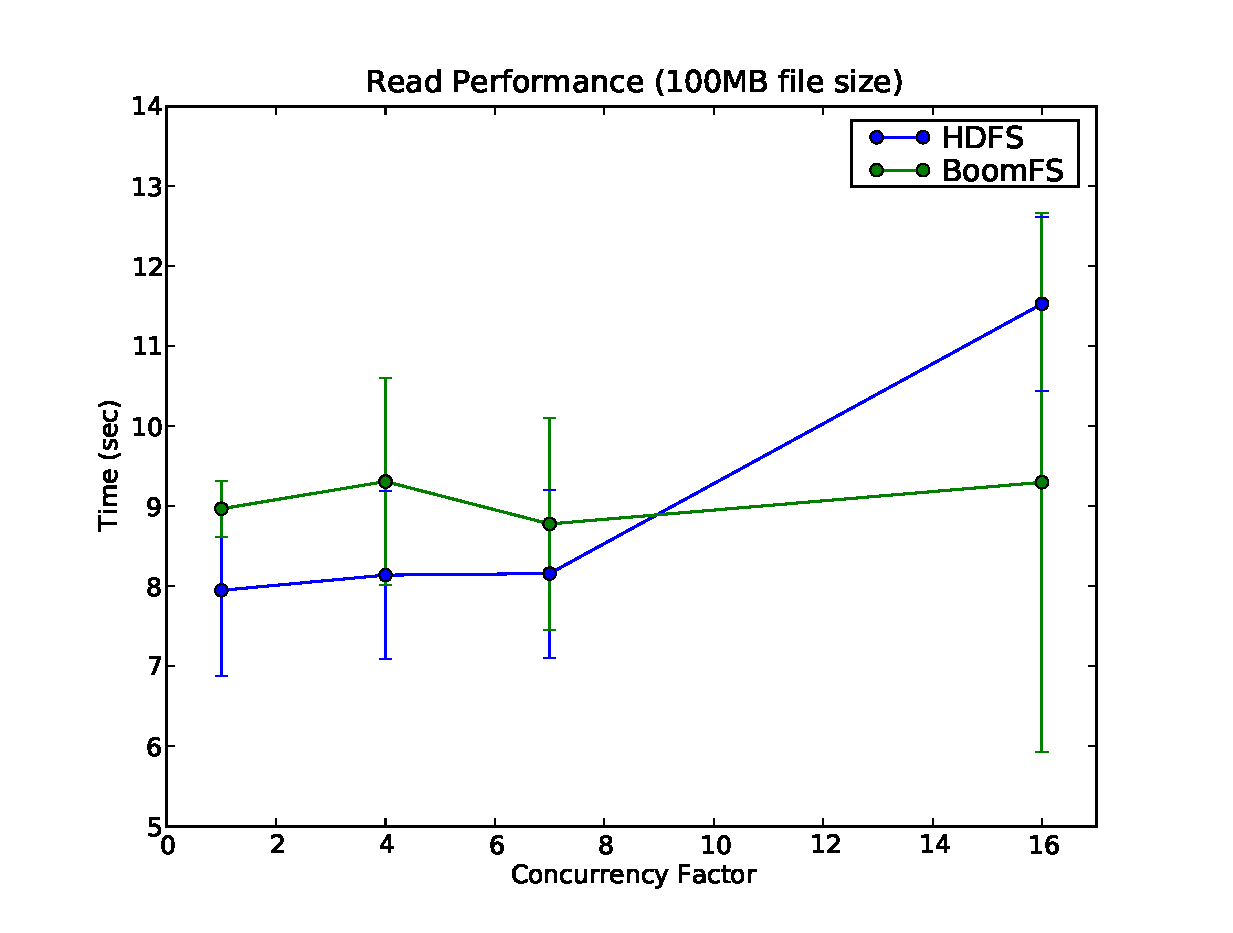
\epsfig{file=figures/big_read_throughput.eps, width=1\columnwidth}
\caption{The components of the BoomFS architecture}
\label{fig:system-arch}
\end{figure}

\subsection{System Overview}
The major components of the BoomFS design are depicted in Figure
\ref{fig:system-arch}. %XXX

Like GFS, BoomFS does not attempt to be a general-purpose distributed
filesystem. Instead, it is designed to perform well for a particular
class of workloads, and to operate on a particular cluster
architecture. We focus on achieving good performance for large
sequential reads and writes. Files are assumed to be very large;
therefore, we choose a large chunk size of XXX. We focus on delivering
high sequential read and write throughput and efficient network
utilization, rather than achieving low latency or efficient usage of
stable storage. Nodes in a BoomFS system are assumed to be unreliable
commodity machines, provisioned with relatively modest resources.
Reliability is achieved by storing multiple copies of each chunk;
scalability is achieved by spreading file system contents over a large
cluster of machines (typically hundreds or thousands).

There are three basic types of nodes in BoomFS: \emph{master nodes},
\emph{data nodes}, and \emph{clients}. Master nodes contain the
canonical description of the structure of the filesystem. The
filesystem is described by a mapping from file names to file
identifiers, and a mapping from file identifiers to the sequence of
chunks that contain the file's content.\footnote{The current prototype
  does not support directories, but this is a relatively
  inconsequential implementation shortcut that we plan to address in
  the near future.} To avoid a single point of failure, our design
allows for multiple master nodes, which are kept in synchrony using a
consensus protocol (currently Paxos~\cite{paxos-made-simple}).

Data nodes are responsible for storing chunks. They have no knowledge
of the structure of the filesystem as a whole, nor even which files
the chunks they store belong to. Each data node periodically sends a
\emph{heartbeat} to the master nodes. This notifies the masters that
the data node is still alive, and contains a list of the chunks
currently stored at the data node. The masters use this information to
update a mapping from chunk identifiers to the set of data nodes that
might be holding that chunk. Note that the canonical description of
the content of a data node resides at the data node itself, not at the
master nodes; the master's copy of this information is updated lazily.

Finally, client nodes represent application programs that wish to read
and write to files stored in BoomFS. We expect that application
programs will interact with the system through a client library that
provides a convenient stream-like abstraction for files stored in
BoomFS. % Other APIs (fuse, hdfs), POSIX

\subsection{Control Path}
To append to a file, a client node begins by contacting one of the
master nodes, and requesting that a new chunk be added to a particular
file.\footnote{In the current prototype, random writes are not
  supported, and each append operation creates a new chunk --- we
  expect that each append will be large enough to justify occupying a
  single chunk. We discuss our plans for relaxing these constraints in
  Section \ref{future-work}.} The master first generates a new chunk
identifier. To ensure that the state of the file system is consistent
across all the masters, the master uses a consensus protocol to ensure
that all masters have agreed to add the new chunk identifier at the
same position in the chunk list for the appropriate file. Once
consensus has been reached, the master sends the new chunk identifier
back to the client, as well as a list of data nodes that might be
appropriate locations for the new chunk.

The client is then responsible for pushing data for the chunk to a
sufficient number of data nodes. There are various policies a client
could use to do this. For example, the client could directly connect
to all the data nodes and send the chunk content itself, or it might
only send the data to a single data node, and instruct that node to
propagate the data onward. Once the chunk content has been completely
received by a data node and written to disk, this fact will be
reflected in the next heartbeat that the data node sends to the
masters. In turn, this will make the data node available for
subsequent operations on the chunk.

To read from a file, a client once again begins by contacting one of
the master nodes to fetch the list of chunks that make up the target
file. For each chunk identifier in the list, the client consults the
master to determine the set of data nodes that have copies of that
chunk. The client then reads the chunk by connecting to one of the
data nodes directly.

\subsection{Data Path}

\subsection{Data Nodes}

\section{System Realization}
\label{system-realize}

\subsection{Software Architecture}

\subsection{Data Representation}

\subsection{Consensus}

\begin{itemize}
\item
  Language integration: what belongs in declarative land, and what in
  imperative land?

\item
  Representation of metadata and data

\item
  Data path implementation

\item
  Use of Paxos as a component
\end{itemize}

\section{Performance Evaluation}
\label{perf-eval}
We validate the applicability of our approach by prototyping a
distributed filesystem based on Google's GFS, and evaluating its
performance and robustness to failure.  Our goal is to achieve
competitive performance on the large append and read workload
characteristic of the GFS environment in spite of the increased
control overhead of our Overlog runtime, and to demonstrate fault
tolerance even when master nodes are lost.  In this section, we
present an evaluation of how successful we were in achieving these
goals.

In the first section, we compare the cost of metadata operations
between our prototype and HDFS, the Hadoop open source implementation
of GFS.  Following this, we simulate a MapReduce sort benchmark,
comparing read and write performance between BFS and HDFS as we scale
the number of concurrent clients and datanodes together.  Finally, we
discuss the various failure modes of the architecture and the impact
of our multi-master extension on these scenarios.

\subsection{Test Environment}
GFS is a proprietary filesystem: we can only speculate about its
implementation based on the documentation that Google has published,
and we cannot evaluate its performance against our own simulated
workloads.  Instead, we used Hadoop, Yahoo's open source
implementation of MapReduce, which includes a distributed filesystem
(HDFS) based on GFS.

We performed our experiments on the Amazon Elastic Compute Cloud, a
virtualized ``utility computing'' environment~\cite{amazon-ec2}.  EC2
provides a convenient and inexpensive testing platform, but this
convenience can come at the cost of high variability in network and
disk performance (LATE paper, EC2).  Hadoop is already well-integrated
with EC2, and instrumenting BFS to handle dynamic address assignment
was trivial.

\subsection{Metadata Operations}
\begin{figure}
\centering
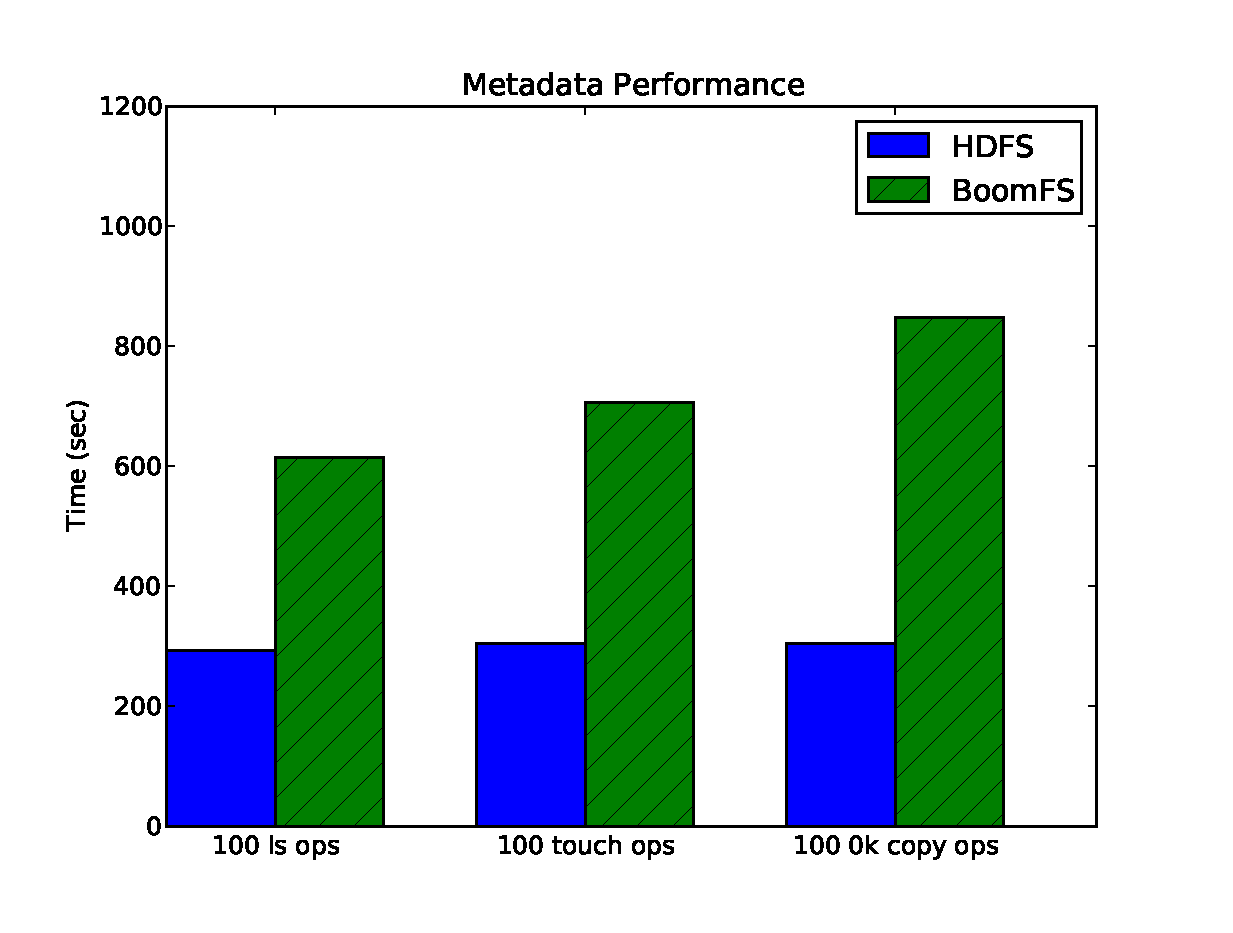
\epsfig{file=figures/metadata_throughput.eps, width=1\columnwidth}
\caption{Performance for metadata operations}
\label{fig:metadata-perf}
\end{figure}

In our first experiment, we compare the latency of metadata operations
affecting the control path.  A directory listing uses the client
protocol and requires a round trip between the client and master and a
lookup on the master, as does touching a file on the filesystem.
Copying a zero-byte file requires two round trips to the master: one
to get a new chunk id for the append operation, and another to request
a link of datanodes who can accept the new chunkid.  (Does hadoop
combine these?  probably, and it would be easy for us to do so).

The results of running 100 of each of these metadata operations are
shown in Figure \ref{fig:metadata-perf}.  As we anticipated, the
overhead of these operations is significantly higher in our
implementation that in HDFS.  This is due in part to client-side
caching, enabled in HDFS and not yet implemented in BFS, although it
would be simple to locally materialize lookup results into relations
that can be queried before visiting the master. (actually, I don't
think we can claim this.  you can't cache lookup results, new file
create requests or new chunk requests!).

\subsection{Sort Benchmark}
Our next experiment evaluates read and write performance under a
typical MapReduce workload.  The sort benchmark of Dean and
Ghemawat~\cite{mapreduce} is a simple and practical test that puts
equal stress on the read and write components of the distributed
filesystem.

The MapReduce specification of sorting is trivial, largely because
sorting (over \emph{some} key) is a side-effect of the framework.
Thus, the map function simply returns the sort key and the entire line
as the key's value, and the reduce function is simply the identity
function.  In an execution of the sort, a single input file is read in
parallel in disjoint sections by all of the mappers, which apply the
hash function and write the bucketed results to their local disks.
The reducers then read these files via RPC calls, apply the built-in
merge sort, and write as many files back to the GFS as there are
reducers.

For the purposes of our experiments, we are interested only in the
costs associated with the parallel reads at the start of the workflow
described above, and the parallel writes described at the end.  Hence,
in our simulation we dispense with the actual sorting, hashing and
crossbarring, and focus merely on the filesystem performance as the
number of concurrent clients and datanodes are scaled up together.
For a given concurrency level D, we provision an EC2 cluster with a
master node and D datanodes, and prime the filesystem by creating D
100MB files with a replication factor of 2.  We then spawn D client
processes (one on each datanode), which read one of the files from the
filesystem, write it to local disk, then create a new distributed
filesystem file and append the contents of the local file to it.
Thus, each client reads (writes) 100MB to (from) the filesystem
concurrently in each sort benchmark, as we vary D.

\begin{figure}
\centering
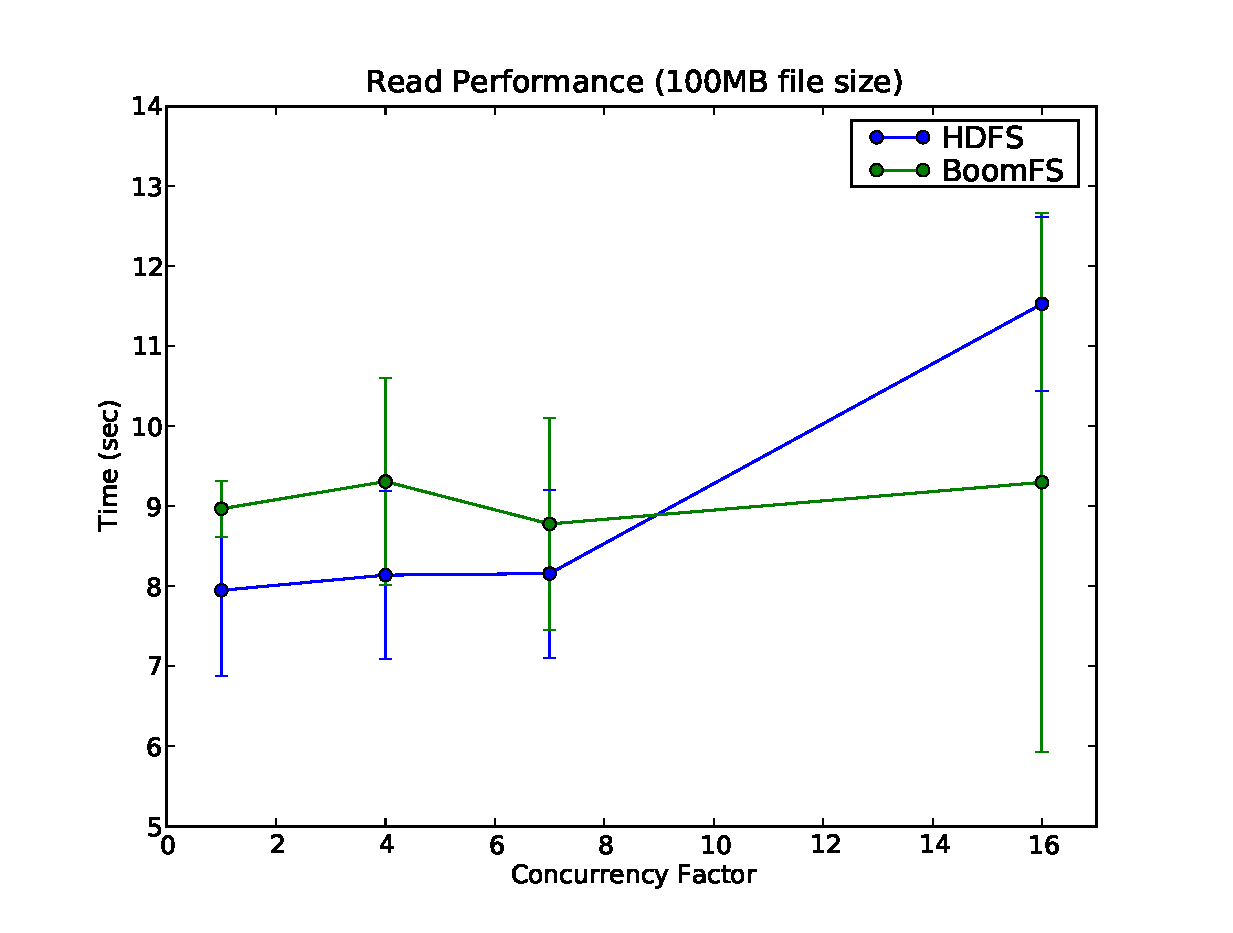
\epsfig{file=figures/big_read_throughput.eps, width=1\columnwidth}
\caption{Sequential read performance for the sort benchmark}
\label{fig:big-read-perf}
\end{figure}
\begin{figure}
\centering
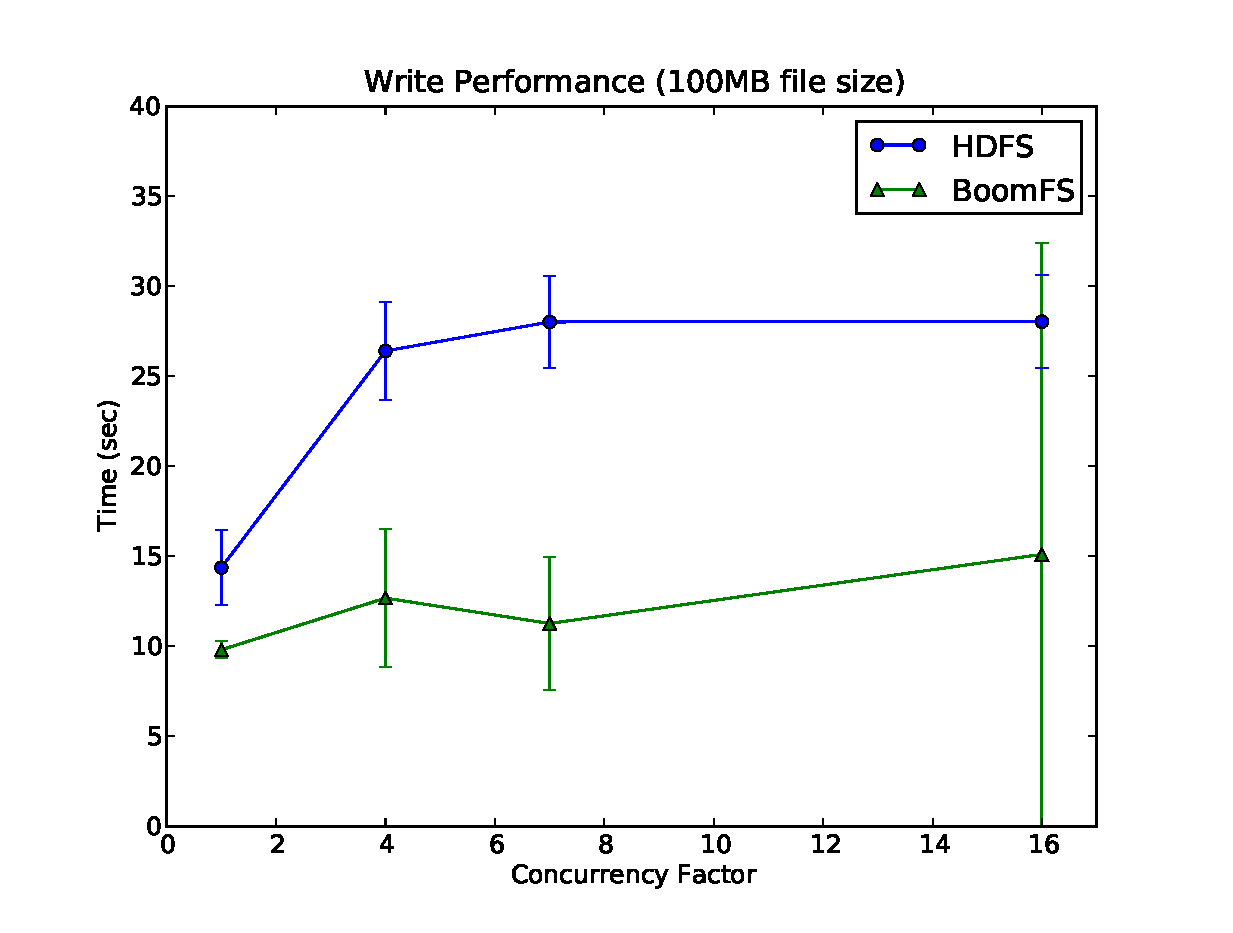
\epsfig{file=figures/big_write_throughput.eps, width=1\columnwidth}
\caption{Sequential write performance for the sort benchmark}
\label{fig:big-write-perf}
\end{figure}
Our results are summarized in Figures \ref{fig:big-read-perf} and
\ref{fig:big-write-perf}.  At lower concurrency levels, BFS is
comparable in read performance and handily outperforms HDFS in write
performance.  This result supports our intuition that the relatively
high cost of metadata operations is quickly amortized by the highly
efficient datapath under the large transfers characteristic of
MapReduce and Hadoop workloads.

In HDFS, read latency increases gradually as load increases, but write
latency reacts very quickly to concurrency, increasing by almost two
times as we increase the number of clients from 1 to 4.  Beyond that
point, HDFS gracefully handles increasing load, with low variance.
BFS shows similar read results, but significantly lower write latency
(less than half that of HDFS, though the variance is higher).  At 16
concurrent clients, the BFS implementation began suffering timeouts.
At this time is is difficult for us to say whether this is due to
issues with queueing in the Overlog runtime implementation, race
conditions or other bugs in the Overlog specification of GFS, or a
problem with the custom data transfer protocol that we implemented.
The variance for x=16 in the graph in Figure 4 reflects the fact that
out of 48 observations, 4 timeouts occurred, resulting in write times
greater than 60 seconds (because our timeout was 60 seconds).  If we
omit those four observations from our results, the mean write response
time is 10.12 seconds.

\subsection{Fault Tolerance}
In the target environment of GFS deployments, namely large clusters of
commodity machines, ``component failures are the norm rather than the
exception.''  In this section we explore several of the failure modes
of the system, and discuss how our integration of a
declaratively-specified Paxos implementation addresses shortcomings in
the original GFS and HDFS design.

\subsubsection{Datanode Failure}
As long as the replication factor is configured to be greater than
two, the loss of a datanode will be transparent to applications using
the system.  The last heartbeats of the lost node will quickly expire
from the soft-state tables on the masters, and clients will no longer
be directed to this server for read or write requests.  The updated
soft state will cause aggregates in the BFS logic to be recomputed,
which in turn cause new migration events to be fired, selecting
another replica as a target for the chunks whose replication factor is
now too low.  GFS and HDFS both use this kind of replication strategy,
though Ghemawat et al. discuss the possible use of other forms of
redundancy, such as parity.

\subsubsection{Datanode Disk Failure}
The effect of this failure is more or less the same as for Datanode
failure, assuming that all the filesystem data is stored on a single
disk.  The datanode will continue to send heartbeats to the master,
but one of these will include a delta record describing the loss of
the files on the disk.  The same chain of inferences described in the
lost datanode scenario described above will fire for these chunks.  It
should be noted that our current prototype will throw an exception
after trying to read from the lost directory, and the datanode service
will stop, resulting in \emph{identical} behavior to the lost datanode
scenario.

\subsubsection{Data Corruption}
GFS and HDFS implement data integrity checking at different
granularities: in HDFS, chunk (called ``blocks'' in HDFS) checksums
are calculated over the entire 64M chunk, while in GFS, a chunk is
subdivided into 64K blocks, each of which has an associated 32bit
checksum.  Our prototype did not implement any integrity checks, but
we plan to add them soon.

\subsubsection{Master Failure}
GFS keeps all filesystem metadata on a single master server to which
all client requests are directed: the mapping is maintained through
the DNS.  Several secondary masters are run in a log replay mode
similar to the log-shipping approach employed by database systems: a
metadata change is not considered committed until the log tail has
been flushed not only to stable local storage, but to all secondary
masters.  This implies the use of a two-phase commit protocol, but the
implementation is not discussed in detail.  If the primary master
fails, the failure must be detected by an external application, which
then remaps the DNS entry to one of the secondaries.
 
HDFS supports the concept of a ``Secondary NameNode'' or backup master
that asynchronously applies log entries to a checkpoint image.  The
primary master supports writing log entries to multiple directories,
one of which can be a remote filesystem such as NFS: a secondary
master can then read the log from this filesystem.  Presumably, this
adds considerable overhead to the performance of the master.
 
In our prototype, a configurable number of masters operate in
lock-step using the Paxos consensus protocol, also implemented in the
Overlog language.

\section{Future Work}
\label{future-work}
\begin{itemize}
\item
  Challenges/difficulties

\item
  Some of the Lincoln vision?

\item
  Cross-layer optimizations

\item
  Continuous query optimization

\item
  Hadoop integration
\end{itemize}

\section{Related Work}
\label{related-work}

\section{Conclusion}
\label{conclusion}

\bibliographystyle{abbrv}
\bibliography{paper}
\appendix
\section{Paxos in Overlog}
\end{document}
